\documentclass[a4paper, 12pt, openright]{book}

% language settings
\usepackage[english]{babel}
\usepackage[T1]{fontenc}

\usepackage[utf8]{inputenc}
\usepackage{textgreek}
%\usepackage{lmodern}
%\linespread{1.5}

\usepackage{fancyhdr} % headers and footers

% figures and positioning
\usepackage{caption}
\usepackage{float}
\usepackage{graphicx}
\usepackage{graphics}
\usepackage{wrapfig}
\usepackage{listing}
%\usepackage{rotating}

% math package
\usepackage{mathtools}
\usepackage{amsthm}
\usepackage{amsmath, amssymb, dsfont, bm}

% tikz figures
\usepackage[usenames, dvipsnames, table, tikz]{xcolor}
\usepackage{tikz}
\usetikzlibrary{shapes, arrows}

% image path
\graphicspath{ {./img/} }

% add support for url and cross-references in PDF output
\usepackage{url}
\renewcommand{\UrlFont}{\color{black}\small\ttfamily}
\usepackage[colorlinks=true, linkcolor=black, citecolor=black, urlcolor=black]{hyperref}

% support for glossary and acronyms
\usepackage[acronym]{glossaries}
\newacronym[plural=MCs,firstplural=Markov Chains (MCs)]{mc}{MC}{Markov Chain}

% Costumization of theorem style
\newtheoremstyle{theoremdd}% name of the style to be used
  {\topsep}% measure of space to leave above the theorem. E.g.: 3pt
  {\topsep}% measure of space to leave below the theorem. E.g.: 3pt
  {\itshape}% name of font to use in the body of the theorem
  {0pt}% measure of space to indent
  {\bfseries}% name of head font %\color{Mahogany}
  { -- }% punctuation between head and body
  { }% space after theorem head; " " = normal interword space
  {\thmname{#1}\thmnumber{ #2}\thmnote{ (#3)}}

\theoremstyle{theoremdd}
% support for counting
\newtheorem{theorem}{Theorem}[section]
\newtheorem{corollary}{Corollary}[theorem]
\newtheorem{lemma}[theorem]{Lemma}
\newtheorem{definition}{Definition}
\newtheorem{remark}{Remark}

% added support for proof parts
\theoremstyle{remark}
\newtheorem{proofpart}{Part}
\renewcommand\theproofpart{\Roman{proofpart}}
\makeatletter
\@addtoreset{proofpart}{theorem}
\makeatother

% specific modification to basic book template of our book document
\renewcommand{\chaptername}{Section}
\addto\captionsenglish{\renewcommand{\chaptername}{Section}}
\renewcommand\qedsymbol{
\includegraphics[width=1.5cm]{occhiali}}
%\renewcommand\qedsymbol{$\square$\itshape QED}


% useful aliases for common employed declarations
\def \beq {\begin{equation}}
\def\eeq{\end{equation}}
\def\bal{\begin{align}}
\def\eal{\end{align}}
\def\prob{\ensuremath\mathbb{P}}
\def\exp{\ensuremath\mathbb{E}}
\newcommand{\Hb}{\mathbb{H}}
\newcommand{\Sb}{\mathbb{\Sigma}}
\newcommand{\U}{\mathbb{U}}
\newcommand{\F}{\mathbb{F}}
\newcommand{\V}{\mathbb{V}}
\newcommand{\A}{\mathbb{A}}
\newcommand{\B}{\mathbb{B}}
\newcommand{\C}{\mathbb{C}}
\newcommand{\E}{\mathbb{E}}
\newcommand{\I}{\mathbb{I}}
\newcommand{\Y}{\mathbb{Y}}
\newcommand{\N}{\mathbb{N}}
\newcommand{\W}{\mathbb{W}}
\newcommand{\Z}{\mathbb{Z}}
\newcommand{\R}{\mathbb{R}}
\newcommand{\X}{\mathbb{X}}
\newcommand{\Pb}{\mathbb{P}}
\newcommand{\Q}{\mathbb{Q}}
\newcommand{\D}{\mathbb{D}}
\newcommand{\Rm}{\mathbb{R^{-1}}}
\newcommand{\J}{\mathbb{J}}

\newcommand{\Fig}[1]{Fig.~\ref{#1}}
\newcommand{\eq}[1]{(\ref{#1})}
\newcommand{\Tab}[1]{Tab.~\ref{#1}}
\newcommand{\Sec}[1]{Sec.~\ref{#1}}
\newcommand{\indep}{\mathrel{\perp\mspace{-10mu}\perp}}
\newcommand{\RN}[1]{ \textup{\uppercase\expandafter{\romannumeral#1}}}

\begin{document}
\section{Go Back N modeling}
%listen to the tape
From a modeling perspective, the packets subsequent to the bad packet are not relevant since we have to re transmit them either (See fig\ref{fig:gbns}). The transmitter will re transmit after two dashed packets so that two slots don't represent throughput since they are going to be rejected. To better understand, we number the packets and suppose to have a two-state Markov Channel:
\beq
\begin{cases}
0 \quad good\\
1 \quad bad
\end{cases}
\eeq
The channel matrix is:
\beq
C = \begin{bmatrix} p_{00} & p_{01}\\p_{10} & p_{11} \end{bmatrix}
\eeq
Every time the source try to retx, it does not do it right after the bad packet but only after a number of packets equivalent to the $R\pi(m)$. Doing so, this does not involve every single slot but some certain slots. The probability that, from the packet num $3$, the packet $4$ is good is a 1-step transmission probability; while the probability that the packet $3$ (coming after the packet $5$) is good is an m-step transmission probability. So we also write down the $m$ step matrix:
\beq
C^m = 
\begin{bmatrix}
p_{00}(m) & p_{01}(m)\\
p_{10}(m) & p_{11}(m)
\end{bmatrix}\footnote{$p_{11}(m)$ is the probability of moving from a bad step to another bad step in $m$ moves}
\eeq
So we can model the protocol assuming error free feedback: (G = good, B = bad).
\begin{figure}
\centering
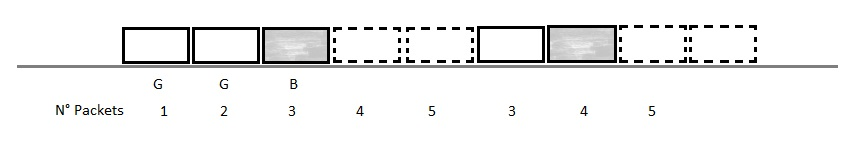
\includegraphics[width = .8\textwidth]{Cri_packets.jpg}
\caption{Go Back N scheme}
\label{fig:gbns}
\end{figure}
\begin{figure}
\centering
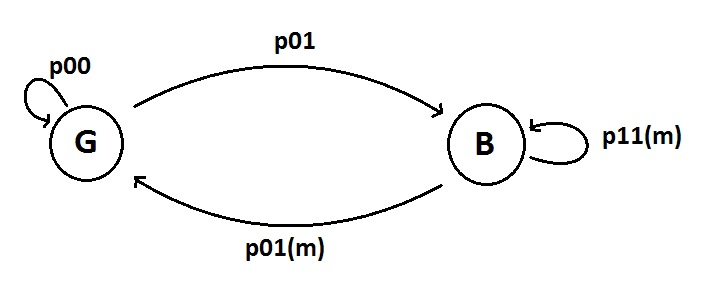
\includegraphics[width = 0.5\textwidth]{Cri_graphGBN.jpg}
\caption{Graph model}
\label{fig:GBN}
\end{figure}
In the model we can describe the behavior of the protocol like: \textit{If the slot is good, then go to the next one, otherwise skip $m-1$ slots and go to the $m^{th}$ one.}\\
With this reasoning it goes that the throughput is expressed as:
\beq
Throughput = \frac{\text{number of good slots}}{\text{total number of slots}}
\eeq
Every visit to state $G$ is $1$ success and every visit to state $B$ is a failure. The respective rewards are: $R_G = 1$ and $R_B = 0$; moreover we associate to $G$ and $B$ different time metrics: $T_{G} = 1$ and $T_{B} = m$, such that we obtain:
\beq
\lim_{t \to \infty}\frac{R(t)}{t} = \frac{\sum_i\pi_iR_i}{\sum_i\pi_iT_i}
\eeq 
And the protocol chain is:
\beq
P = 
\begin{bmatrix}
p_{00} & p_{01}\\
p_{10}(m) & p_{11}(m)
\end{bmatrix}
\eeq
To solve the limit we can find the $\pi$s like:
\begin{align}
\pi_{G} & = \frac{p_{10}(m)}{p_{10}(m)+p_{01}}\\
\pi_{B} & = \frac{p_{01}}{p_{10}(m)+p_{01}}
\end{align}
and insert them in the fraction, not considering the denominators, since they are the same for both the $\pi$s and so they would erase with each other.
\begin{align}
\begin{split}
\lim_{t \to \infty}\frac{R(t)}{t} & = \frac{\pi_GR_G+\pi_BR_B}{\pi_GT_G +\pi_BT_B}\\
& = \frac{p_{10}(m)\cdot1+p_{01}\cdot0}{p_{10}(m)\cdot1+p_{01}(m)}\\
& =\frac{p_{10}(m)}{p_{10}(m)+mp_{01}}
\end{split}
\end{align}
If we suppose an i.i.d. error we obtain:
\beq
\frac{1-\epsilon}{(1-\epsilon)+m\epsilon}
\eeq
Where $1-\epsilon$ is the \textit{P[having a good result | m previous results were bad]}, or better, \textit{P[having a good result]} since we hypothesized the independence of the errors.\\
Now let's try to answer another question: \textit{If we are in state G, how long does it take to us to come back?}\\
The answer is: 
\beq
m_0 = p_{00}\cdot1+p_{01}[1+\frac{m}{p_{10}(m)}]
\label{Formula}
\eeq
Where $m_0$ is the average return time to $G$ and so the inverse of throughput; why? Because as in all semi-Markov processes, if we consider one state, visits to that one state are renewal instants. So the return time from $G$ to itself is a renewal interval and for this specific case, at every renewal cycle we have 1 success and the avg number of successes per unit time is the avg number of successes per cycle, $1$, divided by the average time per cycle. Moreover, once we have obtained the Markov structure we can identify the metrics we need to find.\\
Returning to the expression \ref{Formula}, for the part  inside the rectangular brackets, the expression means that we stay in $B$ for a geometric number of times, which is equal to the average inverse outgoing probability. What we obtain after some algebra\footnote{Fede e Davide this is for you $\heartsuit$} is:
\begin{align}
\begin{split}
m_0 & = 1+\frac{p_{01}\cdot m}{p_{10}(m)}\\
& = \frac{p_{10}(m)+mp_{01}}{p_{10}(m)} 
\end{split}
\end{align}
\\
In the case the feedback has errors, we also need a M.C. for the acknowledgment and to combine it with the previous one, obtaining four states. But the only way to have successful transmission is that both the transmissions works fine:
\beq
C_f =
\begin{bmatrix}
p_{00} & p_{01}\\
p_{10} & p_{11}
\end{bmatrix}
\hspace{10mm}
C_b =
\begin{bmatrix}
q_{00} & q_{01}\\
q_{10} & q_{11}
\end{bmatrix}
\eeq
So the total transmission probability matrix is:
\beq
P =
\begin{bmatrix}
p_{00}q_{00} & p_{00}q_{01} & p_{01}q_{00} & p_{01}q_{01}\\
p_{00}(m)q_{10}(m) & p_{00}(m)q_{11}(m) & p_{01}(m)q_{10}(m) & p_{01}(m)q_{11}(m)\\
\text{$3^{rd}$ and} & \text{$4^{th}$ rows} & \text{can be} & \text{derived}\\
\text{in} & \text{a} & \text{similar} & \text{way}
\end{bmatrix}
\eeq
The state $00$ means $1$ success and $1$ slot, any other state is a failure: $0$ successes and $m$ slots. So I can rewrite the model, defining the vectors $R$ and $T$:
\beq
R =
\begin{bmatrix}
1\\
0\\
0\\
0
\end{bmatrix}
\hspace{20mm}
T =
\begin{bmatrix}
1\\
m\\
m\\
m
\end{bmatrix}
\eeq
and so obtaining the result:
\beq
\lim_{t \to \infty}\frac{R(t)}{t} = \frac{\bar{\pi}\bar{R}}{\bar{\pi}\bar{T}} = \frac{\pi_{00}\cdot 1}{\pi_{00}\cdot1+(1-\pi_{00})m}
\eeq
If now we suppose i.i.d. feedback errors w.p. $\delta$, we obtain the matrix
\beq
C_b =
\begin{bmatrix}
1-\delta & \delta\\
1-\delta & \delta
\end{bmatrix}
\eeq
Moreover, if the feedback channel is i.i.d., we have nothing to remember: regardless of whether the ack is good or bad, we do not care if the transmission was a failure $\rightarrow$ for this case we can use a simplified model with only $3$ states (figure\ref{fig:3states}), where the metrics are:
\beq
R =
\begin{bmatrix}
1\\
0\\
0
\end{bmatrix}
\hspace{5mm}
T =
\begin{bmatrix}
1\\
m\\
m
\end{bmatrix}
\eeq
\beq
p=
\begin{bmatrix}
(1-\delta)p_{00} & \delta p_{00} & p_{01}\\
(1-\delta)p{00}(m) & \delta p_{00}(m) & p_{01}(m)\\
(1-\delta)p_{10}(m) & \delta p_{10}(m) & p_{11}(m)
\end{bmatrix}
\eeq
\begin{figure}[b]
\centering
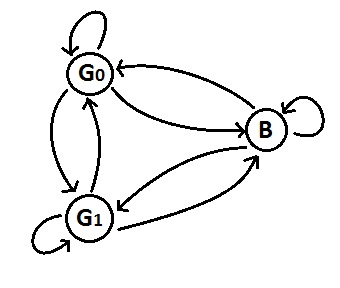
\includegraphics[width=.4\textwidth]{Cri_3states.jpg}
\caption{3-state model}
\label{fig:3states}
\end{figure}
The throughput is:
\beq
\frac{\pi_{G_0}}{\pi_{G_0}+m(1-\pi_{G_0})}
\hspace{5mm}
\bar{\pi} = \bar{\pi}\cdot\bar{P}
\eeq
to obtain it we take:
\begin{align}
\pi_{G_0} & = (1-\delta)(\pi_{G_0}p_{00}+\pi_{G_1}p_{00}(m) +\pi_{B}p_{10}(m))\\
\pi_{G_1} & = \delta(\pi_{G_0}p_{00}+\pi_{G_1}p_{00}(m) +\pi_{B}p_{10}(m)) %Chiedere a Fede
\end{align}
where
\begin{itemize}
\item $(1-\delta)\pi_{G_1} = \delta\pi_{G_0}$
\item $(1-\delta)\pi_{B} = (1-\delta)-\pi_{G_0}$
\item $\pi_{B} = 1-\pi_{G_0}-\pi_{G_1} = 1-\pi_{G_0}-\frac{\delta}{1-\delta}\pi_{G_0} = 1- \frac{\pi_{G_0}}{1-\delta} = \frac{(1-\delta)-\pi_{G_0}}{1-\delta}$
\end{itemize}
and obtaining:
\begin{align}
\begin{split}
\pi_{G_0} & = (1-\delta)p_{00}\pi_{G_0} + \delta\pi_{G_0} p_{00}(m) (1-\delta-\pi_{G_0})p_{10}(m)\\
& = \frac{(1-\delta)p_{10}(m)}{1-(1-\delta)p_{00}-\delta p_{00}(m) +p_{10}(m)}                                      
\end{split}
\end{align}
\beq
1-\pi_{G_0} = \frac{1-(1-\delta)p_{00} -\delta p_{00}(m) + \delta p_{10}(m)}{1-(1-\delta)p_{00}-\delta p_{00}(m) +p_{10}(m)}
\eeq
So the throughput is:
\beq
throughput = \frac{(1-\delta)p_{10}(m)}{(1-\delta)p_{10}(m) + m[1-(1-\delta)p_{00}-\delta p_{00}(m)+\delta p_{10}(m)]}
\eeq
\subsection{Graph reduction}
What if we rewrite the scheme, such that we can reduce it like in figure\ref{fig:GBN}?\\
From a memory point of view it is ok because we do not need to keep memory of the acknowledgments since they are i.i.d; but let's try to understand what happens in terms of success or failure of the acknowledgments:
\\
If we enter state $G$ (we tx a packet and it is succesful)we have:
\begin{itemize}
\item The ack is correct and we found $1$ success in $1$ slot w.p. $1-\delta$;
\item W.p. $\delta$ instead, we count $0$ successes in $m$ slots;
\end{itemize}
This brings us to conclude that in state $G$ we have:
\begin{itemize}
\item $1$ reward w.p. $1-\delta$, $0$ otherwise;
\item $1$ slot w.p. $1-\delta$, $m$ otherwise;
\end{itemize}
About transition probabilities:
\begin{itemize}
\item going to $G$ w.p. $(1-\delta)p_{00}+\delta p_{00}(m)$;
\item going to $B$ w.p. $(1-\delta)p_{01}+\delta p_{01}(m)$;
\end{itemize}
In state $B$ we have:
\begin{itemize}
\item No reward w.p. $1$ and $m$ slots always;
\item We go from there to $G$ w.p. $p_{10}(m)$;
\item And to $B$ w.p. $p_{11}(m)$;
\end{itemize}
So now we have a simplified Markov model where we combine into a single state everything that before was separate. What we obtain is:
\beq
\pi_{G} = \frac{p_{10}(m)}{(\dots)}
\hspace{20mm}
\pi_{B} = \frac{(1-\delta)p_{01}+\delta p_{01}(m)}{(\dots)}
\eeq
Reward and time:
\beq
R =
\begin{bmatrix}
1-\delta\\
0
\end{bmatrix}
\hspace{20mm}
T =
\begin{bmatrix}
1-\delta+\delta \cdot m\\
m
\end{bmatrix}
\eeq
And finally we can estimate the throughput for the system in figure\ref{fig:2states}:
\beq
\lim_{t \to \infty} \frac{R(t)}{t} = \frac{\bar{\pi}\bar{R}}{\bar{\pi}\bar{T}} = \frac{(1-\delta)p_{10}(m)}{(1-\delta+\delta \cdot m)p_{10}(m)+m[(1-\delta)p_{01}+\delta p_{01}(m)]}
\eeq
We just note that the denominator of this expression is equal to the one in the previous throughput expression: to prove it it is necessary to impose:
\begin{itemize}
\item $p_{00} = 1-p_{01}$;
\item $p_{00}(m) = 1-p_{01}(m)$
\end{itemize}
So $1-(1-\delta)p_{00}-\delta p_{00}(m) = (1-\delta)p_{01} + \delta p_{01}(m)$.\\
This result stands out from the fact that the two throughputs are the same quantity but computed by two different models; so we did not reduced the complexity, we just redistributed the quantities.
\begin{figure}
\centering
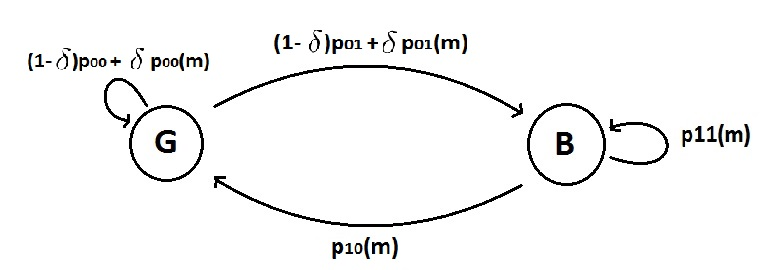
\includegraphics[width=.6\textwidth]{Cri_2states.jpg}
\caption{2-state simplified model}
\label{fig:2states}
\end{figure}
\end{document}